%%%%%%%%%%%%%%%%%%%%%%%%%%%%%%%%%%%%%%%%%
% University Assignment Title Page 
% LaTeX Template
% Version 1.0 (27/12/12)
%
% This template has been downloaded from:
% http://www.LaTeXTemplates.com
%
% Original author:
% WikiBooks (http://en.wikibooks.org/wiki/LaTeX/Title_Creation)
%
% License:
% CC BY-NC-SA 3.0 (http://creativecommons.org/licenses/by-nc-sa/3.0/)
% 
% Instructions for using this template:
% This title page is capable of being compiled as is. This is not useful for 
% including it in another document. To do this, you have two options: 
%
% 1) Copy/paste everything between \begin{document} and \end{document} 
% starting at \begin{titlepage} and paste this into another LaTeX file where you 
% want your title page.
% OR
% 2) Remove everything outside the \begin{titlepage} and \end{titlepage} and 
% move this file to the same directory as the LaTeX file you wish to add it to. 
% Then add \input{./title_page_1.tex} to your LaTeX file where you want your
% title page.
%
%%%%%%%%%%%%%%%%%%%%%%%%%%%%%%%%%%%%%%%%%
%\title{Title page with logo}
%----------------------------------------------------------------------------------------
%	PACKAGES AND OTHER DOCUMENT CONFIGURATIONS
%----------------------------------------------------------------------------------------

\documentclass{article}
\usepackage{fullpage}
\usepackage{alltt}
\usepackage{caption}
\usepackage{float}
\usepackage{amsmath}
\usepackage{courier}
\usepackage{verbatim}
\usepackage[utf8x]{inputenc}
\usepackage{listings}
\usepackage{graphicx}
%Path in Windows format:
\graphicspath{ {images/} }
\usepackage[colorinlistoftodos]{todonotes}
\setlength{\parskip}{1em}
\setlength{\parindent}{0pt}
\begin{document}

\begin{titlepage}

\newcommand{\HRule}{\rule{\linewidth}{0.5mm}} % Defines a new command for the horizontal lines, change thickness here
\newcommand{\immagine[3]{
		\begin{figure}[h]
			\centering
			\includegraphics[width=#3\textwidth]{#1}
			\caption*{#2}
		\end{figure}}}
\center % Center everything on the page
 
%----------------------------------------------------------------------------------------
%	HEADING SECTIONS
%----------------------------------------------------------------------------------------

\includegraphics{logo.png}\\[1cm] % Include a department/university logo - this will require the graphicx package
\textsc{\LARGE Università di Camerino}\\[1.5cm] % Name of your university/college
\textsc{\Large Scuola di Scienze e Tecnologie}\\[0.5cm] % Major heading such as course name
\textsc{\large Informatica (L-31)}\\[0.5cm] % Minor heading such as course title

%----------------------------------------------------------------------------------------
%	TITLE SECTION
%----------------------------------------------------------------------------------------

\HRule \\[0.4cm]
{ \huge \bfseries Sviluppo di una piattaforma di integrazione e omogeneizzazione dati in ambito MES}\\[0.4cm] % Title of your document
\HRule \\[1.5cm]
 
%----------------------------------------------------------------------------------------
%	AUTHOR SECTION
%----------------------------------------------------------------------------------------

\begin{minipage}{0.4\textwidth}
\begin{flushleft} \large
\emph{Autori:}\\
Vincenzo Nucci MAT. 092861 \\
Matteo Tiberi MAT. 092913
\end{flushleft}
\end{minipage}


% If you don't want a supervisor, uncomment the two lines below and remove the section above
%\Large \emph{Author:}\\
%John \textsc{Smith}\\[3cm] % Your name

%----------------------------------------------------------------------------------------
%	DATE SECTION
%----------------------------------------------------------------------------------------

%{\large \today}\\[2cm] % Date, change the \today to a set date if you want to be precise

%----------------------------------------------------------------------------------------
%	LOGO SECTION
%----------------------------------------------------------------------------------------


 
%----------------------------------------------------------------------------------------

\vfill % Fill the rest of the page with whitespace

\end{titlepage}
\section{Obiettivi}
L'obiettivo di questo progetto è la realizzazione di un sistema in grado di omogenizzare dati in ambito MES tramite l'utilizzo di servizi REST. Grazie a questi servizi, una qualsiasi applicazione client è in grado di prelevare dati relativi a macchine utensili, alle quali sono collegati dei sensori che monitorano la produzione e il loro stato di funzionamento. Ci siamo inoltre soffermati sull'integrazione di questa piattaforma con Microsoft Dynamics NAV.
\section{Visione}
Questo progetto è stato realizzato per poter permettere a dati presenti all'interno della Logical System s.r.l., di essere integrati con altre applicazioni client, in particolare con Microsoft Dynamics NAV, software largamente utilizzato all'interno dell'azienda.
\section{Introduzione}
Il progetto prevede lo sviluppo di una piattaforma Java che, tramite un'architettura REST, consente di restituire dati in formato JSON relativi alle letture di sensori collegati a macchinari utensili. La piattaforma prevede inoltre un particolare servizio di subscription con il quale è possibile ottenere i dati in base a una condizione stabilita, mediante l’utilizzo di un message broker. L’interfacciamento alla piattaforma è avvenuto tramite l’utilizzo di Microsoft Dynamics NAV.
\clearpage
\section{Paradigmi, protocolli e strumenti utilizzati}

\begin{itemize}
	\item \textbf{STOMP:} Stomp è un protocollo per lo scambio di messaggi asincrono con architettura client/server.
	Ciò che contraddistingue STOMP è la sua semplicità e interoperabilità: per il fatto che non utilizza
	protocolli binari di codifica dei messaggi ma li invia in formato testuale, può essere anche usato in
	linguaggi come Ruby, Perl e Python.
	\item \textbf{ACTIVEMQ:} ActiveMQ è un broker di messaggistica (Message-Oriented Middleware) che utilizza vari protocolli di trasporto dei messaggi, tra i quali STOMP e OpenWire; permette l’implementazione di code di messaggi con metodologia publisher/subscriber chiamate topic e code chiamate queue nelle quali un messaggio viene letto dal primo client che si connette alla coda\footnote{http://activemq.apache.org/}.
	\item \textbf{REST:} il web server della piattaforma è stato progettato utilizzando un’architettura di tipo REpresentational State Transfer (REST), per indirizzare tutte le risorse secondo una URL unica, rappresentativa ed esplicativa tramite http, e in questo modo fornire una API dinamica e generica\footnote{https://restfulapi.net/}.
	\item \textbf{JERSEY:} è stato utilizzato il framework per servizi REST Jersey\footnote{https://stackoverflow.com/questions/7052152/why-use-jax-rs-jersey}. Jersey è conforme allo standard JAX-RS e per questo facilmente utilizzabile all'interno di un Java server come Grizzly.
	\item \textbf{GRIZZLY HTTP SERVER:} il framework Jersey è in esecuzione all’interno del http server Grizzly. In questo modo è possibile ottenere una soluzione indipendente ed eseguibile su qualsiasi sistema che supporti Java. La scelta di usare un http server anziché un web server è data dalla necessità primaria di scambiare dati tramite protocollo http; rimane comunque possibile pubblicare risorse come pagine web complete di Javascript e CSS.
	\item \textbf{SQLITE:} SQLite è una libreria implementante un database engine. È open source e largamente utilizzata, in quanto strumento leggero ma allo stesso tempo particolarmente potente che consente di costruire un DB ACID completo (comprese tabelle, indici, viste ecc.) ed avere chiamate SQL funzionanti e performanti. Vista la portabilità (in quanto l’implementazione effettiva è un semplice file che rappresenta il database) e la leggerezza, è stato scelto appositamente come strumento per la base di dati per l’amministrazione della piattaforma.
	\item \textbf{APACHE AVRO:} La struttura dei dati che i servizi REST della piattaforma restituisce, è stata definita tramite Apache Avro. Avro è un software che consente, a partire da uno schema, la generazione di classi in vari linguaggi (Java, C\#, C++, ecc...) utilizzate per la costruzione più semplice e formale di JSON. Uno dei motivi per cui è stato scelto Avro è per rendere generale il modello dei dati restituiti: indipendentemente dalle sorgenti dati connesse alla backend, il valore di ritorno di un servizio è sempre in formato Json. in questo modo se è agganciato un file, un database mysql o una websocket, una volta definito lo schema Avro, sarà possibile creare oggetti java che rappresentano i valori di queste sorgenti dati e la restituzione dei dati viene limitata ad una semplice chiamata toString.
	\item \textbf{MICROSOFT DYNAMICS NAV:} Ne verrà trattata una introduzione piu avanti.
	\item \textbf{NAV WEB SERVICES:} NAV permette di integrare applicazioni esterne tramite dei servizi web SOAP, che possono ricevere dati e scriverli in tabelle. questa metodologia sarà usata per implementare il servizio di subscribe anche per NAV. l’interfaccia dei servizi è rappresentata tramite WSDL e grazie a questo è possibile auto-generare il client java, grazie a strumenti appositi.
	\item \textbf{AUTENTICAZIONE NTLM:} è un protocollo di autenticazione di tipo challenge/response presente nei sistemi windows. questo tipo di autenticazione è la stessa usata da NAV e il server dove NAV è in esecuzione è il server in cui si deve autenticare il client che invierà il messaggio al servizio SOAP messo a disposizione da NAV.
\end{itemize}
\clearpage
\section{Architettura Piattaforma}
\begin{figure}[h]
	\centering
	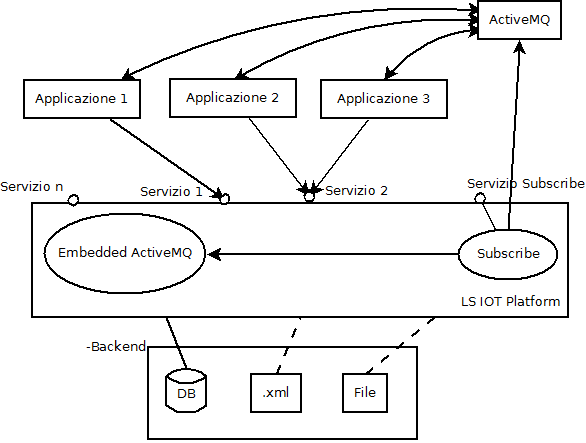
\includegraphics[width=0.8\textwidth]{architettura-piattaforma.png}
	\caption*{Figura 1. Schema della LS IOT Platform}
\end{figure}
La parte principale della piattaforma è il web server con i servizi REST connesso al back end, che nel nostro use-case comprende un singolo database, ma che può essere composto da più sorgenti di dati eterogenee.
Al momento sono disponibili servizi legati all’interfacciamento con il database della Logical System s.r.l. nel quale sono riportate le letture di sensori collegati 24 ore su 24 a dei macchinari e identificati tramite un codice. Nel database è stata inoltre inserita un ontologia in modo da poter descrivere e catalogare in modo formale le informazioni relative ai sensori e alle misurazioni stesse.
In particolare attualmente i servizi disponibili consentono di:
\begin{itemize}
	\item Prelevare la lista dei PLC con la relativa descrizione ed ontologia se presente.
	\item Prelevare l’ultima misura di un sensore.
	\item Prelevare tutte le misurazioni salvate per un dato sensore (questo e i seguenti servizi hanno 2 implementazioni poiché interagiscono con 2 tabelle differenti, in quanto per gli estrusori è presente un’altra tabella a causa dei maggiori parametri da registrare): \begin{itemize}
		\item In base ad una data.
		\item Nell’arco di una settimana a partire dalla data inserita.
		\item Nell’arco di un mese dalla data inserita.
		\item Nell’arco di 2 date da inserire direttamente in input.	
	\end{itemize}
	\item Prelevare le misure da una tabella a scelta a determinate condizioni (sia temporali che di selezione).
\end{itemize}

La struttura dell’URL dei servizi viene elencata da questa tabella:
\begin{center}
	\begin{tabular}{ | l | p{5.06cm} | p{5.06cm} |}
		\hline
		\textbf{Servizio} & \textbf{Input} & \textbf{Output} \\ \hline
		getLastMeasure & \textit{ID} sensore & Ultima misura   \\ \hline
		getMeasureFromTo & \textit{ID} sensore, data \textit{Da}, data \textit{A} & Tutte le misure storicizzate da \textit{Data} a \textit{Data} \\ \hline
		getDetailedMeasureFromTo & \textit{ID} sensore, data \textit{Da}, data \textit{A} & Tutte le misure storicizzate prese dalla tabella degli estrusori, da \textit{Data} a \textit{Data}  \\ \hline
		getMeasureLastMonth & \textit{ID} sensore, Data (\textit{Today}) & Tutte le misure dalla data \textit{Today} a un mese prima \\ \hline
		getMeasureLastWeek & \textit{ID} sensore, Data (\textit{Today}) & Tutte le misure dalla data \textit{Today} a una settimana prima \\ \hline
		getDetailedMeasureLastMonth & \textit{ID} sensore, Data (\textit{Today}) & Tutte le misure dalla data \textit{Today} a un mese prima, degli estrusori \\ \hline
		getDetailedMeasureLastWeek & \textit{ID} sensore, Data (\textit{Today}) & Tutte le misure dalla data \textit{Today} a una settimana prima, degli estrusori \\ \hline
		subscribe & \{\textit{nome applicazione}, \textit{IP applicazione}, \textit{regola},\textit{coda o topic}\} & Misure del sensore caricate come messaggi sulla coda \\ \hline
		unsubscribe & \textit{ID regola} & Annullamento del servizio di subscribe \\ \hline
		getAllPlc & & Lista di tutti i sensori che la piattaforma offre con la relativa ontologia di misure e misurazioni \\ \hline
	\end{tabular}
\end{center}

Per regolare l’accesso ai servizi da parte degli utenti, avere quindi una forma di autenticazione, ogni servizio effettua un controllo nell'header della richiesta che arriva, valutando la presenza di un token. Se il token non è rilevato, la richiesta non viene considerata e un messaggio di errore viene restituito a chi l’ha inviata. \par
Il servizio ActiveMQ è il MOM (Message Oriented Middleware) della piattaforma che funge da tramite tra le applicazioni collegate e i thread della piattaforma per il servizio di subscribe. il collegamento ad una istanza di ActiveMQ esterna alla piattaforma è opzionale, in quanto la piattaforma contiene al suo interno anche una versione embedded del broker. 
\par
Esporre risorse tramite servizi REST permette alla piattaforma di essere indipendente dal tipo di client che si collegano. L’unico requisito che un client deve rispettare per poter ottenere informazioni è il supporto del protocollo http: per poter inviare richieste, collegandosi quindi all’URL che riferisce il servizio, e interpretare il valore di ritorno dell’informazione (nel nostro caso in formato JSON).
\clearpage
\section{Architettura Backend}
\subsection{Descrizione Use Case Aziendale}
Il database con le misurazioni dei sensori è costituito da tre tabelle in cui sono presenti i dati: contengono i valori letti ed elaborati dai controllori logici legati ai sensori collegati ai vari macchinari in produzione che ripetutamente restituiscono i valori letti dai sensori; insieme ad altre quattro tabelle che, se unite con una query, contengono informazioni riguardo l’ontologia delle misure e delle misurazioni. La struttura dei record nelle tabelle dei dati è la stessa per tutti i macchinari, ma l’interpretazione dei valori cambia in base alla tipologia del macchinario e alla famiglia di appartenenza.

Tutte le informazioni relative all’ultima lettura di un sensore vanno nella tabella principale tvmgenio. I dati relativi ad un macchinario che il controllore logico rileva sono inseriti in maniera diretta su un singolo record all’interno di questa tabella; quindi per ogni lettura viene creata una nuova riga contraddistinta dal plc che ha letto i dati (identificato dal proprio canale). 

Le tabelle tvavtest e tvavext sono utilizzate per la storicizzazione dei dati. La prima per la storicizzazione generica di tutte le misurazioni, l’altra per la storicizzazione delle misurazioni dei macchinari estrusori. Per il fatto che contiene molti più valori parametrici aggiuntivi rispetto all’altra tabella, è stata anche definita come dettagliata (i servizi riferiti a questa tabella contengono la parola “detailed”).

\begin{figure}[h]
	\centering
	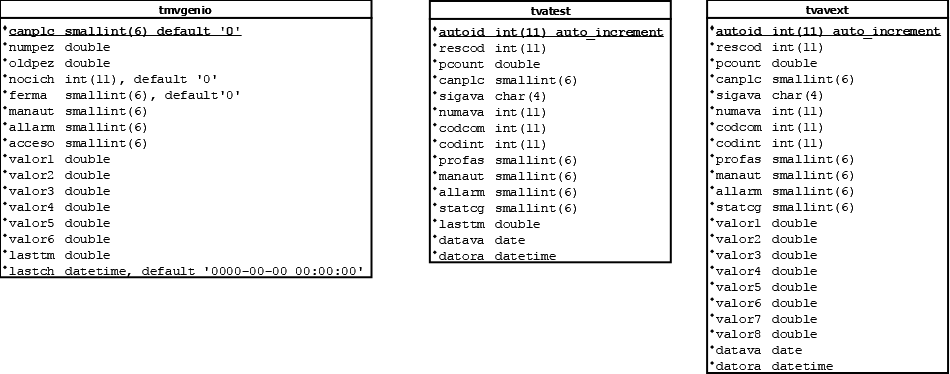
\includegraphics[width=0.8\textwidth]{tabelle-backend.png}
	\caption*{Figura 2.  Struttura delle tre tabelle dei dati}
\end{figure}
Una famiglia di un sensore specifica cosa rappresentano i valori e le misurazioni che sono effettuate. Quindi ad una famiglia è associata una ontologia delle misure e delle misurazioni. Riferita a questa ontologia si ha un servizio apposito che viene utilizzato per presentare il catalogo di sensori offerti dalla piattaforma. Ogni sensore ha la sua lista di campi con la loro ontologia e descrizione. In questo modo chi si registra nella piattaforma, è in grado di informarsi per quali sensori inviare richieste ai servizi REST. Il metodo restituisce un Json contenente tutte queste informazioni e c’è anche una pagina web che converte questo Json in una tabella; in questo modo il catalogo può essere visualizzato sia da una applicazione che tramite browser.
\par
L’ontologia descrive cosa rappresenta ogni campo significativo restituito dal sensore. Normalmente tutti i record hanno un campo che rappresenta il contatore principale dell’informazione che i plc registrano ma questa informazione cambia di significato da un macchinario all’altro. Infatti per i sensori collegati a dei silos, il contatore principale rappresenta la quantità di materiale presente in chili, mentre per gli estrusori rappresenta i metri di tubo prodotti. Perciò un’ontologia è fondamentale per documentare in maniera chiara tutte le informazioni che la piattaforma offre e renderle disponibili agli utenti in modo che possano gestire la scelta di quali sensori usare e per quali servizi.
\clearpage
\subsection{Use Case Diagram}
\begin{figure}[h]
	\centering
	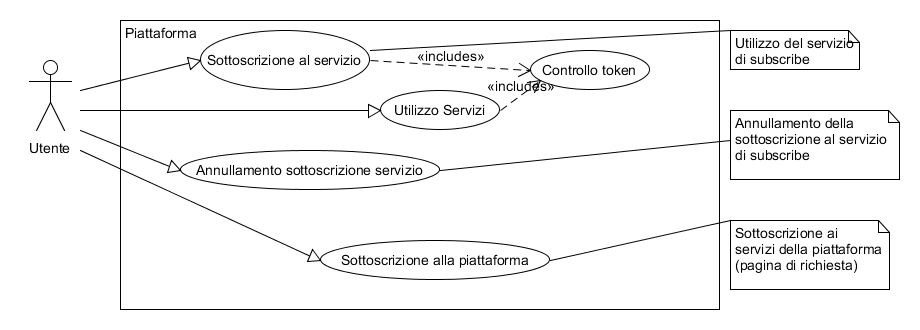
\includegraphics[width=0.8\textwidth]{use-case-utente.png}
	\caption*{Figura 3. Use case lato utente}
\end{figure}
Lo use case lato utente mostra le operazioni che l’utente è in grado di fare nella piattaforma. L’utente può usare i servizi della piattaforma, questa operazione include il controllo del token perchè per poter usare i servizi l’utente deve essere riconosciuto come abilitato. Può usare il servizio di subscribe (sempre se abilitato): questo speciale servizio permette di essere notificati tramite metodologia push riguardo i dati della piattaforma, seguendo largamente il modello publisher/subscriber: appena si verifica la condizione specificata, il servizio informa l’utente inviando il cambiamento dei dati. In altre parole, realizza un servizio di monitoraggio dati in real time per l’utente. La sottoscrizione a questo servizio può essere annullata in qualsiasi momento tramite il servizio unsubscribe. La richiesta del token avviene tramite una apposita pagina web e la sottoscrizione alla piattaforma viene gestita dall’amministratore.

\begin{figure}[h]
	\centering
	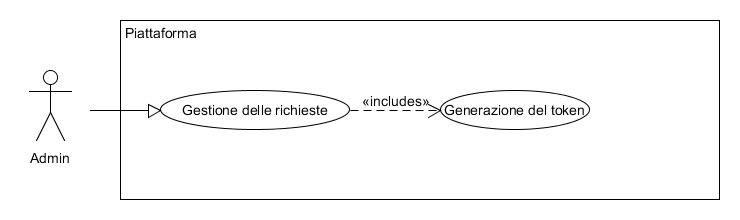
\includegraphics[width=0.8\textwidth]{use-case-admin.png}
	\caption*{Figura 4. Use case lato amministratore}
\end{figure}

Infatti come si vede dallo use case per l’amministratore, è lui che effettua la generazione del token a fronte di una richiesta di sottoscrizione. Una richiesta può anche essere rifiutata.
\clearpage
\subsection{Class Diagram}
Il class diagram risulta essere troppo grande per essere comprensibile all’interno di una singola immagine, perciò ne verranno descritti alcuni frammenti. \par
\begin{figure}[h]
	\centering
	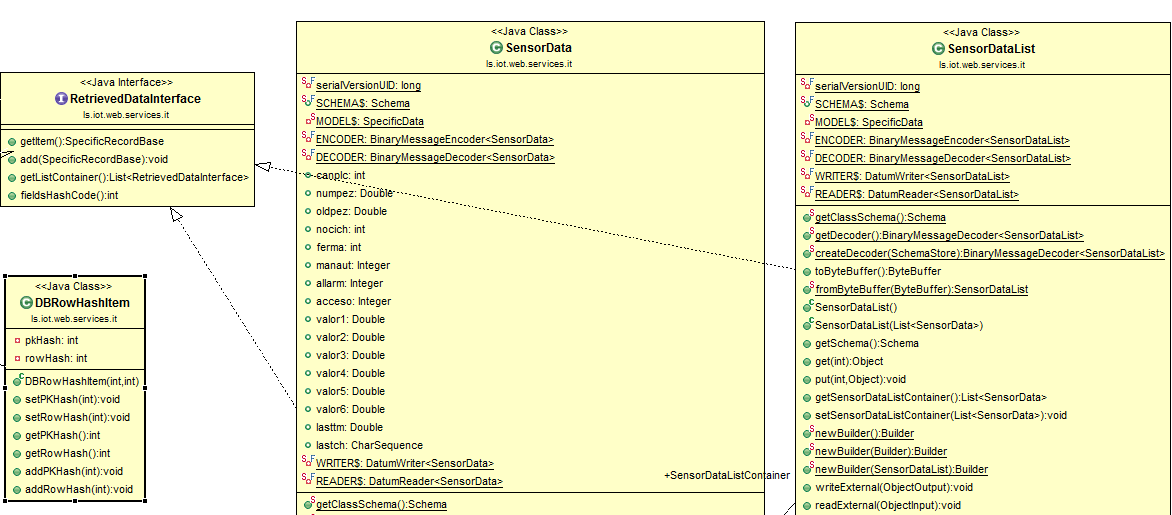
\includegraphics[width=0.8\textwidth]{sensor-data.png}
	\caption*{Figura 5. SensorData e SensorDataList con interfaccia}
\end{figure}
\noindent In questo estratto di class diagram è descritta la classe SensorData che si ottiene compilando lo schema avro. I nomi delle proprietà della classe hanno lo stesso nome dei campi della tabella in modo da avere una relazione univoca tra proprietà dell’oggetto e valore della colonna che si ottiene da una chiamata mysql. In questo modo è possibile inserire i valori ottenuti dal database all’oggetto avro con la chiamata di un solo metodo. SensorDataList è l’oggetto Avro che rappresenta il contenitore (quindi l’array json) di questi oggetti. Si vede infatti la proprietà sensorDataListContainer che è legata da una relazione 0..* con la classe SensorData. Per come è stata implementata la piattaforma ogni oggetto Avro deve avere il rispettivo oggetto lista contenitore. L’interfaccia RetrievedDataInterface rappresenta i metodi che ogni oggetto che si vuole restituire da un servizio REST, deve implementare. I metodi sono getItem per ottenere l’oggetto effettivo, getListContainer e add per ottenere l’oggetto contenitore nel caso in cui l’oggetto effettivo è una lista e per aggiungere un nuovo oggetto alla lista; i metodi per gli oggetti contenitore sono nella stessa interfaccia perchè salendo nella gerarchia delle classi degli oggetti Java generati con Avro, non c’è distinzione tra un oggetto contenitore e un oggetto singolo, entrambi ereditano dalla stessa classe padre; semplicemente un oggetto singolo restituirà null come listContainer e non eseguirà nessuna azione per l'inserimento. il metodo fieldsHashCode è un metodo per ottenere l’hashcode dell’oggetto usando solo i valori delle proprietà, serve per definire se due oggetti sono identici a livello delle sole specifiche proprietà definite all’interno del metodo. Usando RetrievedDataInterface è possibile interagire con qualsiasi sorgente dati nella backend purchè venga definito un oggetto Avro che rappresenti i dati che contiene. 
\par
Avere una rappresentazione dei dati come schema Avro permette di raggruppare tutti i possibili dati che una piattaforma può restituire come oggetti RetrievedDataInterface. In questo modo la piattaforma può evolvere e gestire diversi schemi Avro di differenti oggetti.
\clearpage
\begin{figure}[h]
	\centering
	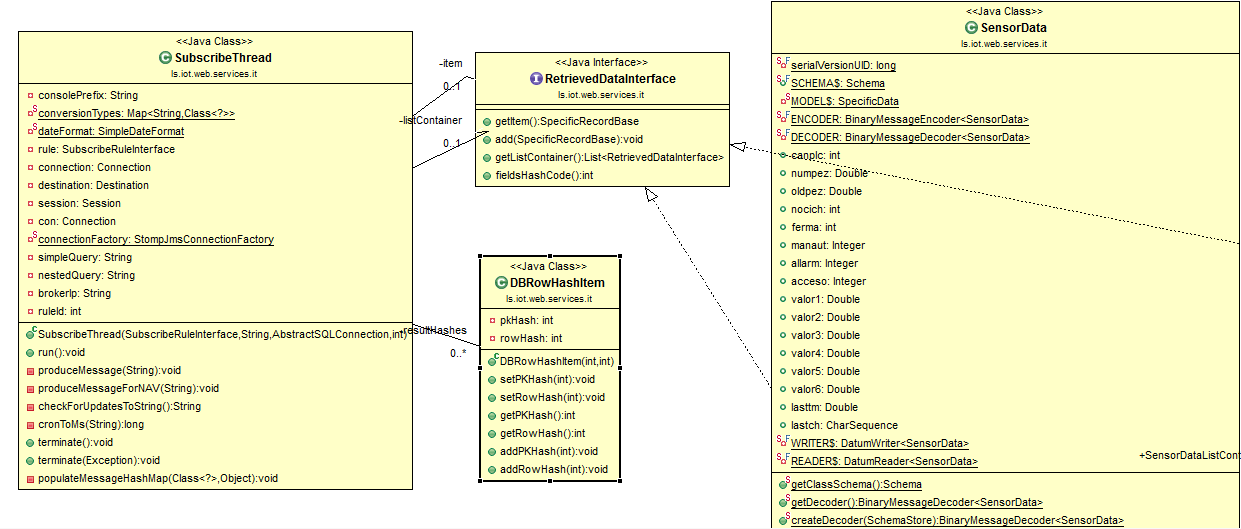
\includegraphics[width=0.8\textwidth]{subscribe-thread.png}
	\caption*{Figura 6. SubscribeRule e SubscribeThread con interfaccia}
\end{figure}
Questo estratto di class diagram rappresenta l’oggetto thread che viene lanciato quando un client effettua una sottoscrizione al servizio push della piattaforma. Il thread contiene tutte le informazioni necessarie per eseguire query alla sorgente dati, rappresentata dall’oggetto connessione, che sono: la regola che deve eseguire ad ogni intervallo di tempo (intervallo CRON); riferimenti al broker di messaggistica dove andrà a  scrivere i nuovi dati che sono cambiati.
\par \vspace*{2em}
\begin{figure}[h]
	\centering
	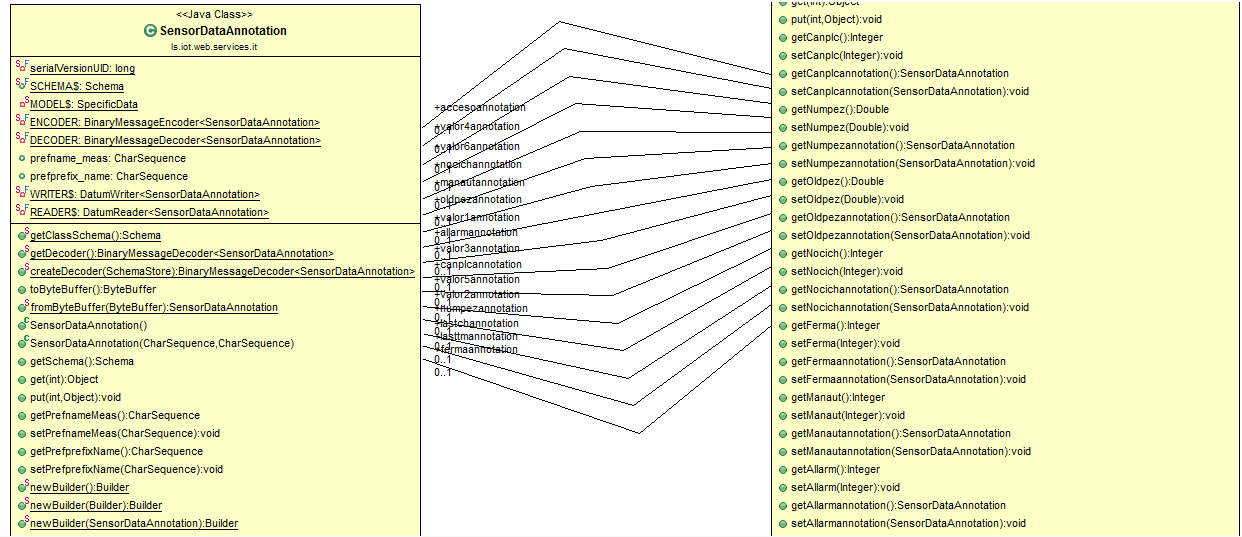
\includegraphics[width=0.8\textwidth]{sensor-data-annotation.png}
	\caption*{Figura 7. SensorDataAnnotation}
\end{figure}
Questo estratto di class diagram rappresenta l’oggetto annotazione che è presente negli oggetti Avro del caso d’uso aziendale. L’annotazione rappresenta l’ontologia legata alla misura (e non alla misurazione) che ogni singola proprietà dell’oggetto rappresenta. i campi che costituiscono una annotazione sono il nome dell’ontologia di riferimento e il suo ID.
\clearpage
\begin{figure}[h]
	\centering
	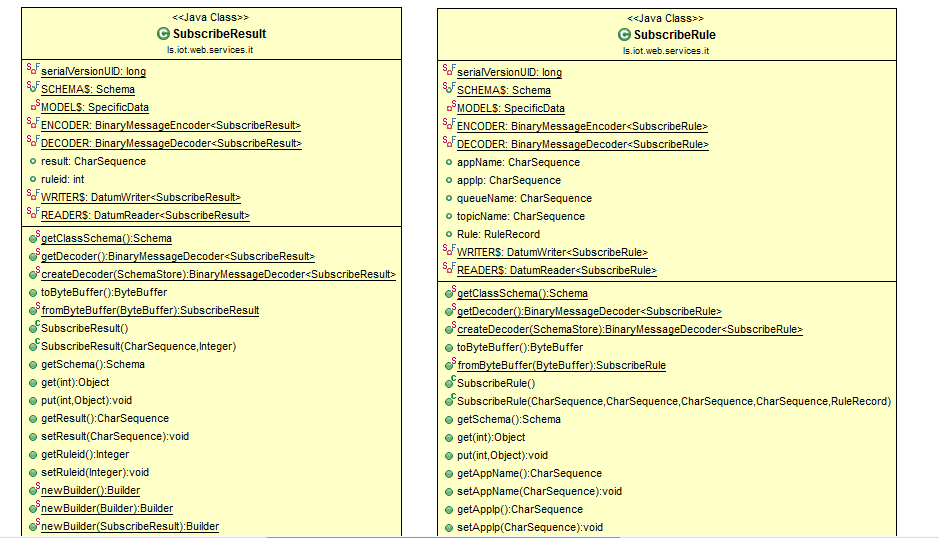
\includegraphics[width=0.8\textwidth]{subscribe-result.png}
	\caption*{Figura 8. SubscribeRule e SubscribeResult}
\end{figure}
Questo estratto di class diagram rappresenta gli oggetti della regola espressi con lo schema Avro che permette di definire la query sql con oggetti annidati; insieme all’oggetto che viene restituito ad un client ad indicare l’esito della sottoscrizione al servizio di subscribe. L’oggetto regola ha come proprietà il nome dell’applicazione, l’ip dell’applicazione, la coda o topic in cui dovrà andare a scrivere e la regola, ovvero la query SQL. L’oggetto SubscribeResult ha come proprietà semplicemente un messaggio result e un valore intero che rappresenta l’ID che il server ha associato alla sua regola. Questo identificativo viene usato poi nel caso in cui l’utente vuole annullare la sottoscrizione al servizio di subscribe.
\par \vspace*{2em}
\begin{figure}[h]
	\centering
	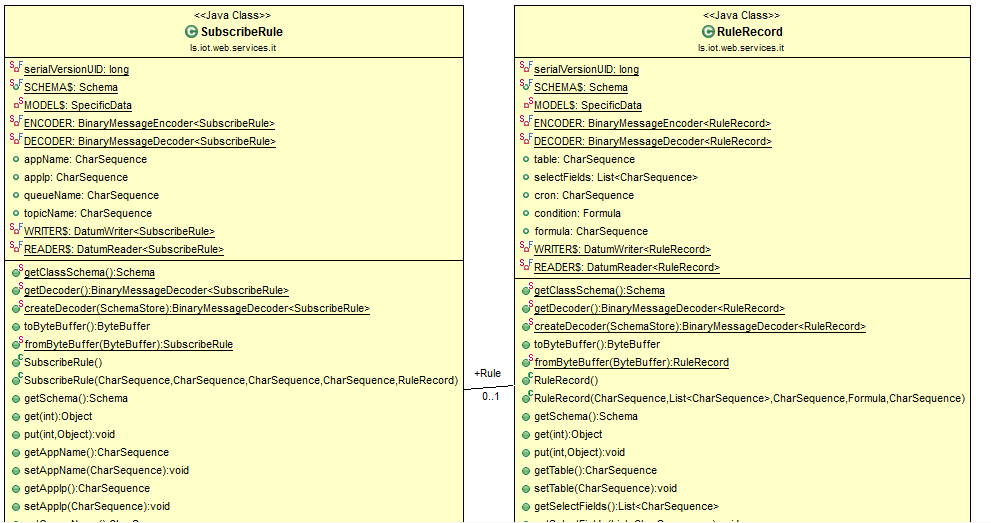
\includegraphics[width=0.8\textwidth]{rule-record.png}
	\caption*{Figura 9. SubscribeRule e RuleRecord}
\end{figure}

La regola contiene: l’array dei campi del database dei quali si vuole essere notificati, ovvero l’utente viene notificato solo se viene registrato un cambiamento per quei campi che ha richiesto; la tabella dove effettuare la query; il CRON in formato stringa e la clausola where che è rappresentata da condition e formula. Condition rappresenta la definizione della where in maniera complessa, formata da più oggetti differenti e annidati; mentre formula rappresenta la where in una semplice stringa scritta a mano. Questa suddivisione della where è necessaria per il nostro caso d’uso, perchè in Microsoft Dynamics NAV non si può creare una finestra di input in cui ogni operazione viene aggiunta in maniera incrementale, perciò la query viene indicata direttamente come stringa.
\par \vspace*{2em}
\begin{figure}[h]
	\centering
	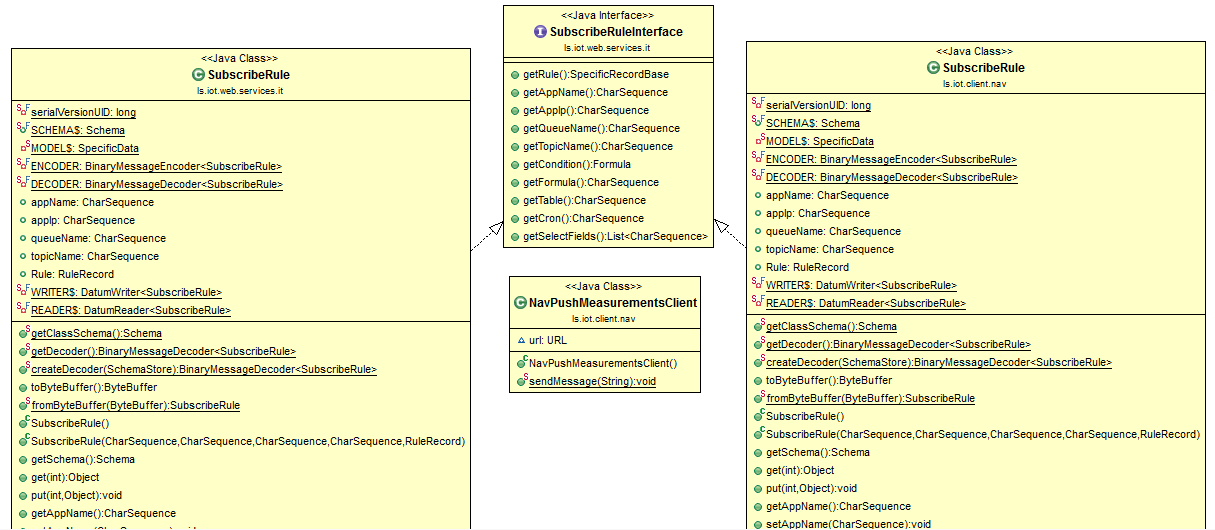
\includegraphics[width=0.8\textwidth]{rules.png}
	\caption*{Figura 10. SubscribeRule generale e per NAV con interfaccia}
\end{figure}
Per rendere la regola generica e implementabile in ogni situazione è stata definita un’interfaccia. Questa interfaccia implementa i metodi necessari per rappresentare una regola, quindi metodi che restituiscono i campi della query, la tabella, la where, ecc…
\par
La comodità di questa soluzione sta nel fatto che l’implementazione della where non dipende dallo schema Avro. Il problema che ha fatto nascere il bisogno di questa interfaccia è il seguente. La piattaforma utilizza lo schema della regola complesso in cui la where può essere definita come formula o come condition, e condition è un valore opzionale. Anche se condition è opzionale, quindi può non essere presente (nota del sito di avro), nell’atto pratico deve esserlo con il valore di default\footnote{https://stackoverflow.com/questions/22939391/generating-an-avro-schema-with-optional-values}, nel Json che viene inviato al servizio di subscribe. Microsoft Dynamics NAV usa uno schema diverso da quello della piattaforma, una versione semplificata della regola in cui la condition non è definita. Questo significa che se la piattaforma implementa lo schema complesso della regola, quando riceve richieste di subscribe da parte di un client Navision, non è in grado di processare la richiesta in quanto nello schema non è presente il valore condition. In questo modo basta fare in modo che il thread accetti regole di tipo SubscribeRuleInterface per riuscire a gestire regole sia di Navision che di altre applicazioni.
\clearpage
\begin{figure}[h]
	\centering
	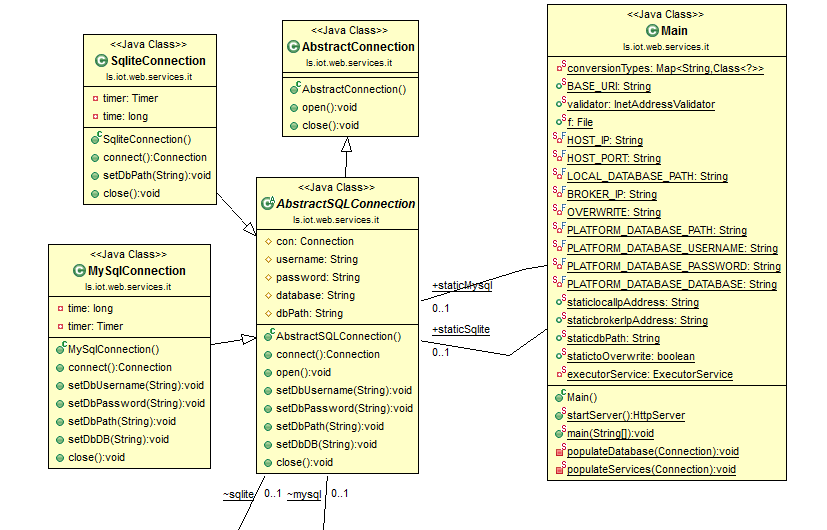
\includegraphics[width=0.8\textwidth]{main.png}
	\caption*{Figura 11. Classe astratta per gestire le connessioni}
\end{figure}

Questo estratto di class diagram rappresenta la gestione delle connessioni nella piattaforma. Per poter estendere la backend a qualsiasi sorgente dati, è stata definita una classe astratta AbstractConnection che ha come metodi generali open e close, di primaria funzione per ogni sorgente dati come file o database. Questi metodi possono essere quindi sovrascritti in base al corretto funzionamento desiderato, da classi figlie che rappresenteranno l’implementazione concreta della connessione. Per il nostro use case è necessario inoltre avere connessioni a database SQL perciò è stata definita la classe astratta AbstractSQLConnection che rappresenta una connessione qualunque ad un database SQL: ha come proprietà il path in cui si trova il database, username e password per collegarsi e il nome del database. Questa classe così definita rappresenta connessioni sia a database Mysql, dove solitamente ci si collega ad un server, sia connessioni di tipo Sqlite dove il database è un file su disco. Le implementazioni fisiche sono quindi differenziate per MySQL e Sqlite a cui sono state aggiunte un timer per fare in modo di chiudere la connessione dopo 10 minuti di inutilizzo.
\clearpage
\section{Struttura Dati Json}
L’utilizzo del framework Avro ha questi vantaggi\footnote{http://blog.cloudera.com/blog/2011/05/three-reasons-why-apache-avro-data-serialization-is-a-good-choice-for-openrtb/}:
\begin{itemize}
	\item Avro può gestire in maniera dinamica i dati, utile in situazioni dove lo schema dei file non è noto al momento della compilazione. La gestione dinamica non richiede di generare una classe da utilizzare all’interno del programma, ma avviene tramite un GenericRecord. In questo modo i dati possono essere inseriti con dei metodi put. Un piccolo svantaggio del GenericRecord è che l’utilizzo dei metodi put/get richiede di specificare di quale campo si vuole inserire o richiedere il valore; 
	\item Mentre nella gestione dei dati con l’utilizzo di classi che contengono lo schema (code-generation)\footnote{https://stackoverflow.com/questions/30277442/what-does-code-generation-mean-in-avro-hadoop}, i metodi get/put che permettono di accedere ai dati sono auto esplicativi ed esiste un metodo per ogni campo definito nello schema. Inoltre i metodi di get e put accettano come parametro anche il nome del campo e quindi il vantaggio dell’utilizzo di Avro si è visto nella popolazione dell’oggetto che rappresenta i valori dei sensori, avendo come nomi di proprietà gli stessi campi della tabella. 	
\end{itemize}
La struttura che abbiamo definito per rappresentare i dati della tabella tvmgenio è la seguente.
{\fontfamily{pcr}\selectfont
\lstinputlisting[breaklines]{sensor-data.txt}
}

Vengono ripresi gli stessi campi del record nel database MySQL, in modo da avere una relazione diretta con il nome e inserire quindi i valori tramite la proprietà put con un singolo metodo.
\par
Inoltre sono presenti i campi delle annotazioni, che sono altri oggetti contenenti i valori di ID e nome dell’ontologia della misura. L’ontologia delle misure nello schema Avro è chiamata annotazione ed è un valore opzionale.
L’annotazione cambia il comportamento dei servizi della piattaforma, infatti se viene richiesta, la query di interrogazione dei dati e il popolamento della lista contenitore cambiano. Per come è strutturato il database mysql aziendale, quando l’annotazione viene richiesta, lo stesso oggetto della tabella viene ripetuto più volte per ogni annotazione che ha e per evitare di trasferire tutto il result set in una variabile in memoria e poi effettuare un accorpamento per risultati simili, si è scelto di fare tutto mentre si scorre il result set tenendo conto del valore precedente dell’oggetto: nel caso in cui l’oggetto è lo stesso, i campi vengono saltati e si passa a popolare solo l’oggetto annotazione che non viene inserito all’interno del nuovo oggetto ma in quello precedente. In questo modo si ha sempre una sola versione dello stesso oggetto con le annotazioni aggiornate. Per questa modalità di inserimento e gestione si è dovuto fare un controllo aggiuntivo sul fatto di essere arrivati all’ultima riga del result set, perché inserendo il valore precedente quando non corrisponde al valore attuale, succede che arrivati all’ultimo elemento questo non verrà mai inserito.
\par
Gli schemi Avro per le altre tabelle SensorHystoricalData e SensorHystoricalDataExt sono fatte allo stesso modo di SensorData.
\clearpage
\subsection{Struttura della regola}
Lo schema Json che rappresenta una regola per il servizio di Subscribe è il seguente. 
{\fontfamily{pcr}\selectfont
	\lstinputlisting[breaklines]{subscribe-rule.txt}
}
Come già detto, nello schema Json che il servizio di subscribe riceve, viene specificato il nome e l’indirizzo IP dell’applicativo che richiede la sottoscrizione, il nome della coda o del topic del message broker e la regola, un oggetto chiamato SubscribeRule che contiene tutte le informazioni riguardo la regola di subscribe. Queste informazioni sono: i campi della tabella che l’utente vuole popolati nei messaggi di ritorno, la query che il thread deve effettuare sul database, la tabella che deve essere interrogata e un CRON che indica l’intervallo di tempo ogni quanto il thread si deve attivare.
\clearpage
Un generico Json che potrebbe essere inviato al servizio di Subscribe da parte di un client è il seguente.
\begin{figure}[h]
	\centering
	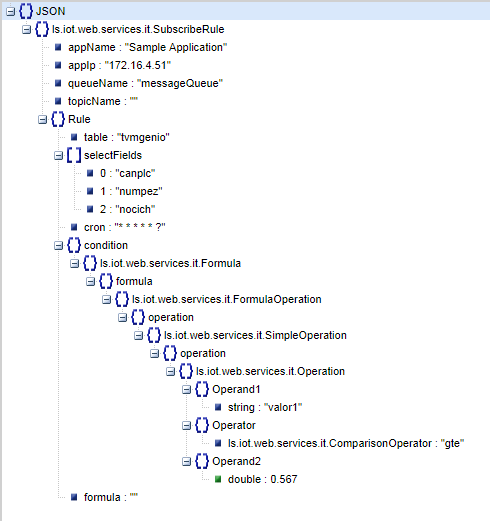
\includegraphics[width=0.4\textwidth]{subscribe-json-1.png}
	\caption*{Figura 12. SubscribeRule in formato Json}
\end{figure}
\par
In questo schema le operazioni SQL sono descritte da enum che hanno come simboli tutti i possibili operatori. Ci sono gli Operatori di Confronto, gli Operatori Aritmetici, gli Operatori per le operazioni bit a bit, gli Operatori Binari e gli Operatori che si applicano ad altre sub-query. Il punto di partenza della condition è un oggetto Formula che ha un oggetto FormulaOperation. Da questo oggetto FormulaOperation si differenziano operazioni che comprendono operatori logici binari come and, or, ecc... ; operazioni che comprendono operatori logici che si applicano ad altre sotto-query come any, some, ecc… e infine operazioni singole che comprendono operatori di confronto, aritmetici, ecc… tra due operandi.
\par
Una versione schematizzata della struttura di una query è la seguente.
\begin{figure}[h]
	\centering
	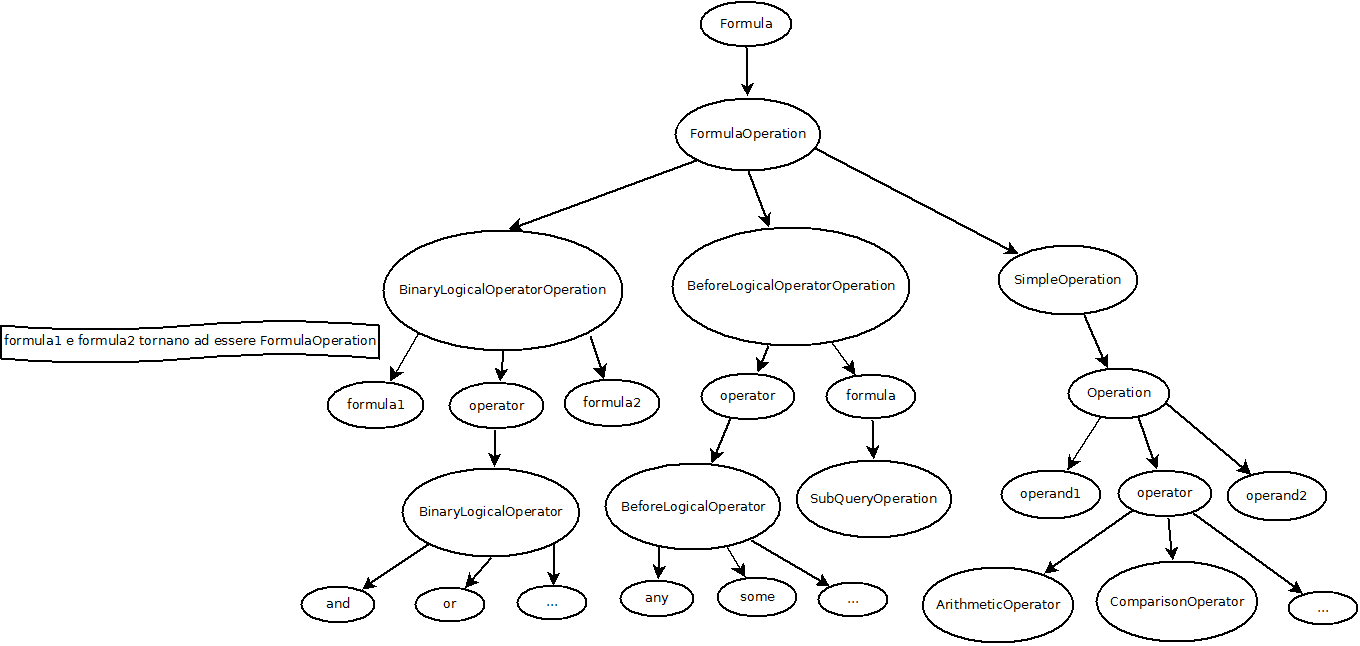
\includegraphics[width=0.8\textwidth]{struttura-query-tree.png}
	\caption*{Figura 13. Schema ad albero della definizione di condition}
\end{figure}
\clearpage
Mentre lo schema Avro di una SubscribeRule inviata da parte di un client Microsoft Dynamics NAV è questo.
\begin{center}
		{\fontfamily{pcr}\selectfont
			\lstinputlisting[breaklines]{subscribe-rule-nav.txt}
		}
\end{center}
A differenza dello schema principale, in questo esiste solo il valore formula nello schema. E questo è un possibile Json che potrebbe essere inviato al servizio di subscribe da parte di un client Navision.
\begin{figure}[h]
	\centering
	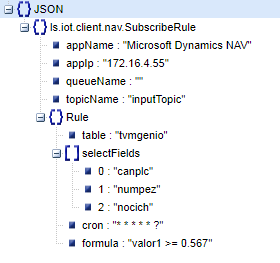
\includegraphics[width=0.4\textwidth]{subscribe-json-2.png}
	\caption*{Figura 14. SubscribeRule in formato Json proveniente da NAV}
\end{figure}
\par
In Avro i nomi consentiti per i campi possono iniziare soltanto con le lettere a-z sia maiuscole che minuscole e l’underscore, perciò l’implementazione di uno schema che abbia l’operazione come valore key e gli operandi come value risulta impraticabile, inoltre i nomi degli operatori logici e aritmetici sono stati codificati secondo il loro nome sempre per questa limitazione dei nomi.
\par
Usiamo Avro anche per la regola di Subscribe in modo da avere una soluzione robusta e sicura, ed avere un controllo immediato per quanto riguarda la ricezione di Json malformati: nel momento in cui il Json arriva al server, è in formato stringa senza nessun controllo. Viene poi convertito in un byte array, il formato serializzato che Avro può interpretare, seguendo proprio lo schema Avro. In questo modo si riesce poi a istanziare un oggetto che rappresenta una regola di subscribe. In questo modo si può elaborare una regola, quindi creare un thread sul server, creare una coda nel broker,… prendendo i dati dalle proprietà get dell’oggetto anziché effettuare il parsing manualmente dalla stringa Json.

\section{Servizio di Subscribe}
Il servizio di subscribe è composto da un oggetto Executor che organizza un “pool” di thread, di numero indefinito, la quale esecuzione verrà gestita dall’executor stesso. Un thread rappresenta l’oggetto che ha il compito di gestire una singola regola ricevuta dal servizio. La gestione dei thread rimane possibile grazie al metodo submit dell executor che restituisce un Future<?>. Questo tipo di oggetto rappresenta lo stato di esecuzione di un thread e grazie a questo è possibile fermarlo in qualsiasi momento chiamando il metodo terminate. Cosi è come funziona il servizio di Unsubscribe. La struttura dati che gestisce il Subscribe è una hashmap che associa all’id della regola ricevuta dal servizio il thread che andrà a gestirla. 

Il server una volta che riesce a mandare in esecuzione correttamente un thread, restituisce un Json che indica se l’operazione è andata a buon fine. Lo schema di questo oggetto SubscribeResult è il seguente.
\begin{center}
		{\fontfamily{pcr}\selectfont
			\lstinputlisting[breaklines]{subscribe-result.txt}
		}
\end{center}
Questo oggetto definisce un messaggio result che indica il termine dell’operazione e un intero che rappresenta l’ID associato alla regola che il client potrà poi usare per annullare la sottoscrizione di questa regola al servizio.
Il thread per capire se i dati sono cambiati nel database, mantiene una struttura dati che contiene l’hashcode dei record che ottiene dalla query. Questo hashcode è mantenuto da un oggetto che salva in due proprietà diverse l’hash della chiave del record e l’hash del corpo del record. Questa gestione permette di fare in modo che la posizione del valore hash nella hashmap non sia legato con la posizione del record nel risultato della query. In questo modo se il contenuto di un record cambia, indipendentemente dalla sua posizione nel result set, viene aggiornato nella hashmap seguendo i valori di chiave primaria (che sono fissi e non cambiano per definizione). \newline
Nel Subscribe per applicazioni Microsoft Dynamics NAV non è stato possibile utilizzare lo stesso sistema di una coda ActiveMQ, per la mancanza di NAV di poter avere un servizio sempre attivo che andasse a leggere nella coda. Per questo Navision ha un servizio ad hoc nel quale il thread che gestirà la sua sottoscrizione andrà a scrivere i dati che gli sono pervenuti dalla query al database e dei quali ha notato un cambiamento e NAV aggiungerà questi nuovi dati nella sua tabella dei valori real time. Il client Java per inviare messaggi al servizio di NAV è stato auto-generato tramite la WSDL messa a disposizione proprio dal servizio di NAV. Inoltre nel connettersi al servizio, bisogna autenticare il client Java con un profilo che abbia i permessi di scrivere nel servizio NAV. L’autenticazione avviene a livello di profilo windows tramite il protocollo NTLM. \newline

\section{Token Authentication}
Un client per poter utilizzare un servizio deve essere abilitato e per farlo deve fare richiesta di un token, tramite una apposita pagina. Nella pagina le informazioni da inserire sono il nome dell’applicazione, il suo IP, le credenziali che si vorranno usare per accedere alla pagina personale di gestione dei servizi e la sua email, tramite la quale verrà notificato del suo token. Una volta inviata la richiesta, questa verrà inserita all’interno di un database di amministrazione, che con la tabella Requests riferirà tutte le richieste di token inviate dagli utenti. Il token è una stringa di caratteri alfanumerica che rappresenta l’abilitazione dell’utente all’utilizzo dei servizi della piattaforma. È generato tramite la classe UUID di java in modo da garantire l’univocità di ogni token.
\par
Una pagina di gestione permette ad un amministratore di abilitare l’utente ad usare i servizi, quindi genererà un token specifico per quel client, che verrà notificato in qualche modo della generazione del suo token.
Una volta ottenuto il token, l’utente che si è sottoscritto ad usare i servizi deve impostarlo nell’header di ogni richiesta. È proprio grazie a questo che un client riesce ad utilizzare i servizi della piattaforma. Il controllo dell’header che arriva avviene sullo stesso database delle richieste ma in una altra tabella contenente tutti i token che sono stati rilasciati agli utenti. Se un token che arriva ad un servizio rientra nei token registrati, allora chi vuole usare quel servizio può farlo.
\par
Con il sistema del token è stato implementato anche un modo per tenere traccia delle statistiche di utilizzo dei servizi da parte degli utenti. Nel database è presente una tabella dei servizi contenente i nomi con il rispettivo ID di tutti i servizi che sono presenti nella piattaforma. Avendo associato un ID ad ogni servizio, è possibile tenere delle variabili per ogni ID: quando un utente effettua una richiesta di abilitazione, sceglie quali servizi vuole attivare e in questo modo popola una lista che contiene l’id di ogni servizio che vuole abilitare. Quando la richiesta viene accettata, questa lista è inserita anche nella tabella delle sottoscrizioni attive e ne viene generata una simile con tutti i valori a zero. Questa altra lista rappresenta l’utilizzo dei servizi nella lista dei servizi attivi, dove la posizione di un ID è la stessa nella lista degli utilizzi. In questo modo quando un utente che ha una lista di servizi attivi come questa [1,2,3] effettua una chiamata al servizio 3, nella lista degli utilizzi, il contatore nella terza posizione viene incrementato di 1 [0,0,1]. questo avviene automaticamente nella stessa funzione che controlla se un client è abilitato ad usare un servizio.
\clearpage
\section{Gestione degli errori}
\subsection{Schema Avro}
\begin{center}
		{\fontfamily{pcr}\selectfont
			\lstinputlisting[breaklines]{exception-handler.txt}
		}
\end{center}

Per dare un feedback all’utente in caso di utilizzo errato dei servizi, viene restituito il messaggio di errore dell’eccezione che viene generata dal sistema, notificando l’utente di cosa è successo. A questa eccezione è associato un numero che rappresenta l’hashcode della classe, in questo modo si definisce un codice di errore per categoria: le NullPointerException hanno il loro codice, cosi come le IllegalArgumentException, ecc… e un livello di errore in base alla gravità di cosa è successo.

\section{Database Amministrativo}
La piattaforma ha come basi di dati principale un database Sqlite che contiene informazioni riguardo le richieste di token che sono arrivate; regole che sono attualmente registrate e quindi in esecuzione; utenti attualmente abilitati ad usare la piattaforma il loro utilizzo dei servizi. \newline
Questa immagine mostra, ad esempio, la gestione delle regole di subscribe attualmente attive.
\begin{figure}[h]
	\centering
	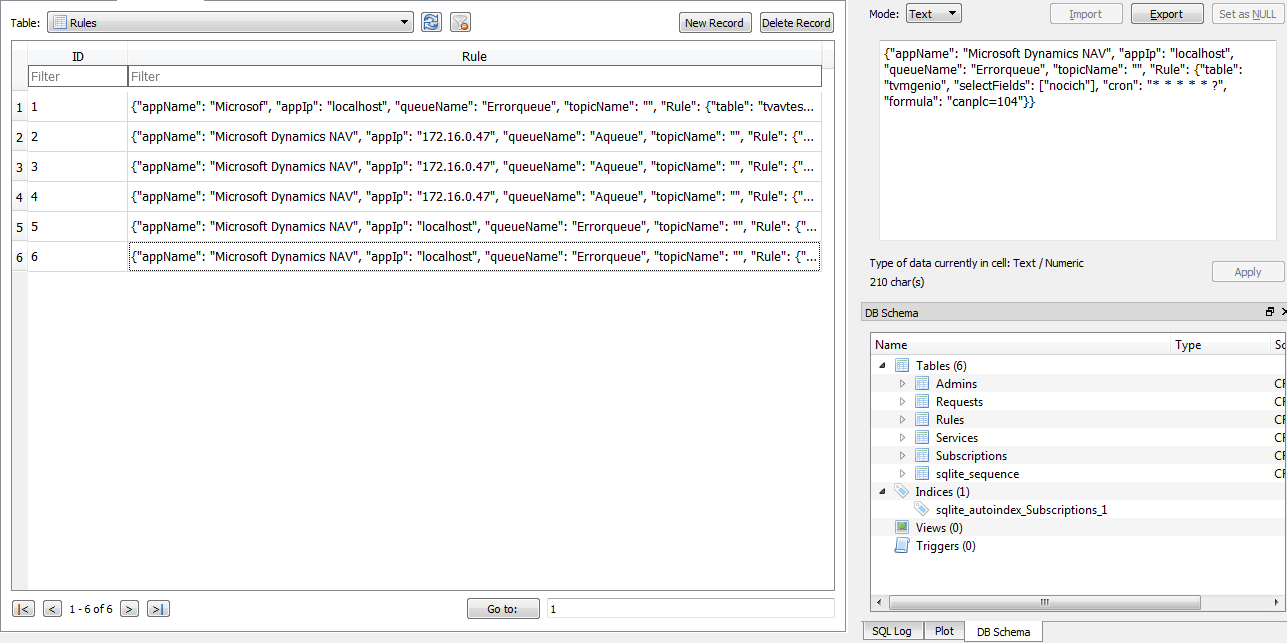
\includegraphics[width=0.8\textwidth]{db-rules.png}
	\caption*{Figura 15. Screenshot della gestione delle Rules}
\end{figure}
\clearpage
Il database amministrativo della piattaforma ha, codificata nel metodo principale che viene eseguito quando mandato in esecuzione, lo scheletro delle tabelle. In questo modo la piattaforma genera il suo ambiente di lavoro ogni volta che viene avviata in un nuovo contesto in cui il database non è presente. La piattaforma è così portabile e indipendentemente da dove viene lanciata, generando ogni volta il database con un amministratore di default. \newline
La piattaforma ha anche questa funzionalità: per rispettare la struttura di un login in ambiente client/server, anche in assenza di un server php, una hashmap di sessioni regola il login degli utenti. Come session ID viene usato l’hashcode di username e password concatenate e la sessione contiene username e password di chi effettua il login in modo da poter inviare al client un cookie contenente il session ID e permettergli di visualizzare il contenuto delle pagine. Il cookie ha durata di 1 ora e vale su tutto il dominio /ls della piattaforma.

\section{Espressioni CRON}
Le espressioni cron sono utilizzate in ambienti Unix-like per eseguire una determinata operazione in un determinato intervallo di tempo (per esempio ogni minuto 10 di ogni giorno). Utilizza una sintassi particolare formata nel modo seguente:
\begin{center}
	{\fontfamily{pcr}\selectfont
		\lstinputlisting[breaklines]{espressione-cron.txt}
	}
\end{center}
Dove l’anno è facoltativo. In cron è possibile inserire dei caratteri speciali come il ? (indicante nessun valore) e * (indicante ogni valore ammesso dall’intervallo).

\section{Architettura Lato Client}
Nell’architettura generale è previsto l’utilizzo di un client che è sempre attivo e rimane in attesa dell’embedded broker activemq che lo notifica con nuovi dati. Nel momento in cui questa applicazione viene interfacciata con Microsoft Dynamics NAV si hanno delle difficoltà in quanto non vi è la possibilità di ricevere dati in maniera push direttamente ma è necessario passare per un ulteriore step: l’utilizzo di un webservice SOAP da NAV\footnote{https://blogs.msdn.microsoft.com/freddyk/2010/01/19/connecting-to-nav-web-services-from-java/} con il quale è consentito esternare codeunit, pagine e query. In questo modo tramite il WSDL è possibile compilare automaticamente un client per quel webservice e interagire direttamente con quel servizio. Sarà così possibile la ricezione di dati sempre aggiornati successivamente alla sottoscrizione del servizio in base ad una regola specificata dall’utente senza dover necessariamente utilizzare tecniche di pooling (con cui continuo a chiamare costantemente il server per sapere se vi sono nuovi dati).
\subsection{Breve Introduzione su Microsoft Dynamics NAV}
Microsoft Dynamics NAV è un software gestionale pubblicato da Microsoft. Esso consente alle imprese una completa gestione della contabilità e del magazzino tramite tabelle e pagine, dispone di un sistema centralizzato con autorizzazioni in modo che solo determinati utenti possano accedere a determinate aree di lavoro. NAV è suddiviso in client e ambiente di sviluppo (development environment) : nel client è possibile inserire e visualizzare dati, mentre nell’ambiente di sviluppo è possibile inserire codice C\textbackslash AL e costruire oggetti che poi verranno utilizzati nel client. Sia client che development environment lavorano su uno stesso servizio il quale deve essere disponibile su un server NAV. \newline
Gli oggetti costruibili nell’ambiente di sviluppo di Microsoft Dynamics NAV sono: 
\begin{itemize}
\item Tabelle (alla base, le quali contengono i dati che il client mostrerà).
\item Pagine (che consentono una vista sui dati di una o più tabelle).
\item Query (che consentono di effettuare operazioni di selezione sui dati delle tabelle).
\item Codeunit (classi in C\textbackslash AL code utilizzabili per compiere particolari operazioni sui dati).
\item XMLport (che consentono di importare file XML).
\item Report (che permettono di visualizzare e stampare dati dalle tabelle) .
\item Menusuite (i quali permettono di visualizzare un menu a lato nell’ambiente di sviluppo, per esempio per raggruppare gli oggetti necessari per un determinato sviluppo).
\end{itemize}
Oltre che nelle codeunit, all’interno di questi oggetti è inoltre possibile inserire del codice C\textbackslash AL in corrispondenza di determinati “trigger”, ovvero punti in cui un determinato evento è verificato. 
\section{Client C\#}
Per interagire con l’interfaccia LSIoT che fornisce servizi REST è necessario a sua volta avere un client in grado di consumare questi servizi. Nel nostro caso ci siamo occupati di interfacciare Microsoft Dynamics NAV con questa piattaforma sviluppata in Java ed è stato necessario estendere le funzioni del suo ambiente in quanto NAV non può direttamente utilizzare servizi REST. Con NAV è infatti possibile l’utilizzo di librerie realizzate in C\# e compilate come .dll. In questo modo è stato creato un client in grado di consumare servizi REST e utilizzarlo a sua volta all’interno dell’ambiente Navision, con successivo trattamento dei dati ricevuti.
\clearpage
\subsection{Class Diagram}
\begin{figure}[h]
	\centering
	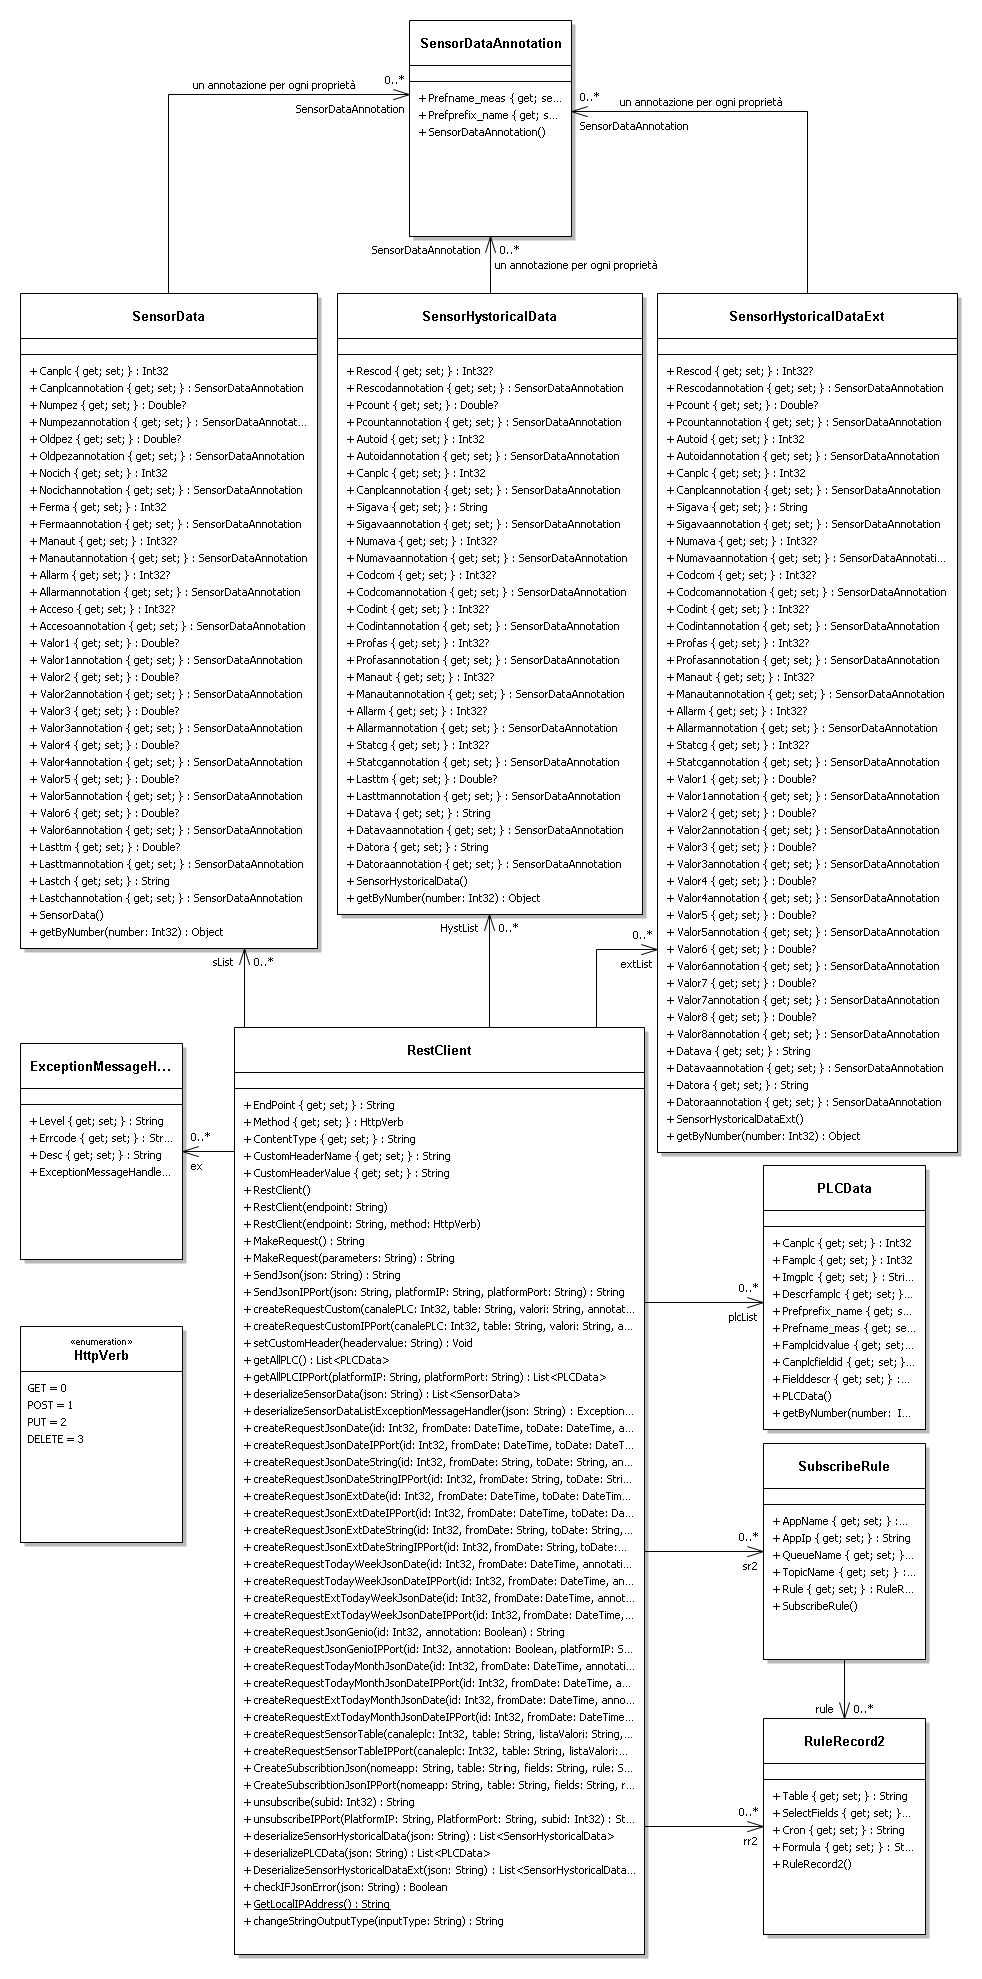
\includegraphics[width=0.47\textwidth]{class-diagram-client.png} \newline
	\caption*{Figura 16: Class Diagram Client C\#}
\end{figure}
\clearpage
Come si nota dal class diagram il client è composto da varie classi che sono utilizzate da un'unica classe RestClient, la quale si occupa di effettuare le vere chiamate ai servizi. Ogni metodo della classe RestClient relativo all’utilizzo dei servizi REST ha tra i parametri ciò che deve passare alla piattaforma tramite richiesta http in base al servizio, la connessione alla piattaforma e la deserializzazione della risposta. Inoltre ognuno di essi ha una seconda definizione che presenta tra i parametri anche la possibilità di inserire IP e porta della piattaforma. Questa scelta è stata fatta in quanto se si ci si vuole collegare ad un indirizzo diverso rispetto a quello impostato nei vari metodi (per esempio nel caso in cui la piattaforma cambi indirizzo IP) risulta possibile senza dover necessariamente cambiare il codice C\# e ricompilare dunque la dll. Per poter utilizzare questi servizi, è tuttavia necessario effettuare una sottoscrizione alla piattaforma. La sottoscrizione avviene tramite sito web e una volta iscritti viene assegnato un id della relativa sottoscrizione e, se la sua sottoscrizione è accettata, un token al richiedente che dovrà utilizzare quando chiama i vari servizi (dovrà essere inserito nell’header del messaggio http). Per quello che riguarda il servizio di subscription vengono anche inseriti altri dati oltre al nome del client richiedente e all’indirizzo come la coda su cui si vuole operare in activemq, ogni quanto tempo si vuole la ricezione dei dati aggiornati (tramite formula CRON), la condizione con la quale si vuole richiedere i dati (espressa praticamente come clausola where della chiamata SQL e la tabella dalla quale si andranno a ricevere i dati). In questo caso i dati verranno inviati al client a seconda delle condizioni stabilite dal subscription e, come per tutti i servizi vengono inviati in formato JSON.


Oltre ai metodi strettamente legati alla piattaforma vi sono anche metodi per prendere in maniera dinamica il proprio indirizzo IP e metodi di controllo del JSON, che potrebbe arrivare contenente semplicemente un errore con il tipo, codice e descrizione. Sia per l’errore che per il messaggio di sottoscrizione sono stati elaborati schemi avro e classi generate con i relativi metodi di deserializzazione. 

Le classi utilizzate da RestClient non sono state create a mano ma sono state generate automaticamente e formalmente dal software Apache Avro. 

Avro è utlizzato solitamente in ambiente java, ma è disponibile anche una versione per .NET, la quale tuttavia, genera delle classi con meno metodi rispetto alla controparte in Java, che nonostante ciò sono comunque molto utili per il loro scopo principale. Nonostante infatti non sia possibile nativamente generare il JSON direttamente da una classe generata da uno schema, queste classi rendono molto più semplice l’interazione con metodi e attributi di tali oggetti. Inoltre l’approccio formale garantisce che non vi siano differenze nei nomi degli attributi del JSON in quanto le classi sono generati dal medesimo schema.

Il client è stato utilizzato inizialmente come client REST C\# a se stante per testare l’utilizzo dei servizi forniti dalla piattaforma e successivamente è stato integrato, dopo aver generato la dll, nell’ambiente Navision. Il testing e la generazione della libreria avvengono sulla stessa soluzione ma in 2 progetti diversi, in modo da utilizzare i metodi dall’esterno, in maniera simile a quanto avviene su NAV.

Per quello che riguarda la connessione Il client REST usa il metodo MakeRequest dove si crea un istanza di WebRequest utilizzando l’indirizzo del servizio REST come URI (identificato come endpoint). Questa istanza viene convertita ad HttpWebRequest (in quanto chiamare HttpWebRequest.create corrisponde a chiamare create da WebRequest). Successivamente si imposta il metodo, la lunghezza e il tipo del contenuto e infine l’header http (necessario per passare il token utilizzato nella sottoscrizione ad un servizio). Si procede poi con la creazione dell’oggetto response, il quale conterrà la risposta (tramite chiamata del metodo request da getResponse,  si controlla che lo status code di risposta sia il 200 (ok) e si crea un oggetto Stream dal quale si andrà a leggere con uno streamreader ciò che è contenuto nel body della risposta (nel nostro caso il Json contente i risultati dal DB).
\clearpage
Per quello che riguarda l’invio di dati in formato JSON è stato creato un metodo con il quale si procede allo stesso modo del metodo MakeRequest ma stavolta si utilizzano 2 stream, uno streamwriter per mandare il mio JSON per la sottoscrizione al servizio “push” alla piattaforma e uno streamreader per ricevere la risposta della piattaforma contente un json con il risultato della sottoscrizione e l’id relativo.

Nonostante sia generalmente consigliato l’utilizzo di httpClient, è stato utilizzato HttpWebRequest\footnote{http://www.diogonunes.com/blog/webclient-vs-httpclient-vs-httpwebrequest/}. httpClient è più semplice e costruito sopra httpwebrequest per diminuire la quantità di codice da scrivere per effettuare una richiesta, ma non è compatibile con tutte le versioni del .NET Framework. Dato che il client NAV ha la possibilità di utilizzare metodi relativi alla versione 4.0 del .NET Framework per maggiore stabilità con NAV dunque si è adottata questa soluzione, ma in futuro non è escluso che si possa passare a all’utilizzo di httpclient.

Una volta che i dati in formato JSON arrivano correttamente al client C\# è dunque necessaria una deserializzazione dei dati tramite opportune classi corrispondenti al JSON di arrivo. Per la deserializzazione è stato utlizzato JSON.NET, un framework disponibile per ambiente .NET ed installabile tramite pacchetti NuGet. Questo framework consente di deserializzare e serializzare JSON con semplici e brevi istruzioni.


\begin{figure}[h]
	\centering
	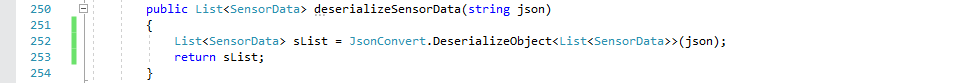
\includegraphics[width=0.8\textwidth]{deserialize.png}
	\caption*{Figura 17: Utilizzo del framework nella deserializzazione di un oggetto generato dallo schema avro.}
\end{figure}

Con questo framework è inoltre possibile la costruzione di JSON tramite codice con l’utilizzo di appositi metodi dell’oggetto JsonWriter (come ad esempio WriteStartObject, WritePropertyName, WriteValue ecc.). Proprio con questi metodi e con gli oggetti delle classi generati è stato possibile costruire il JSON per il servizio di subscribe.

In Microsoft Dynamics NAV si hanno 2 metodi per utilizzare le dll generate dagli utenti: mettendole sul client o sul server. Dato che, se una libreria è posizionata sul server, una sua modifica o sostituzione richiede un riavvio dell’intero servizio, inizialmente essa è stata messa su client e una volta verificato che i servizi funzionassero in maniera corretta è stata direttamente caricata sul server in cui viene lanciato il servizio. Oltre al vantaggio che chiunque operi su quel servizio possa utilizzare la dll, mettere il file su server comporta anche dei vantaggi prestazionali. Nonostante sia semplice importare una libreria di classi vi sono comunque dei vincoli da rispettare: Nell’ambiente di sviluppo di NAV per esempio si hanno dei problemi con l’override dei metodi (non visualizza le altre implementazioni) e I tipi inoltre non sono gli stessi anche se solitamente è disponibile una conversione implicita (es. Int $\rightarrow$ Integer (NAV), double $\rightarrow$ decimal (NAV), String $\rightarrow$ Text (NAV), bool $\rightarrow$ Boolean(NAV)). Tutto il lavoro di manipolazione del JSON inoltre è fatto dentro la dll, in quanto non è possibile utilizzare, in maniera corretta, direttamente sul development environment di NAV i metodi di JSON.NET.

Inizialmente per il push dei dati sempre aggiornati si era pensato di eseguire un metodo che facesse da “client” (chiamato sempre dalla dll) sempre in ascolto in NAV e che, ricevuti i dati, li andasse direttamente a mettere in una tabella dedicata. Purtroppo, non è possibile implementare nell’ambiente NAV direttamente una soluzione di questo genere in quanto durante l’esecuzione di un metodo il Client Navision non è utilizzabile (il quale rimane bloccato nel PC dell’utente finché non è terminata l’esecuzione di questo metodo e questo potrebbe risultare in un blocco non trascurabile in un ambiente lavorativo). Come alternativa però, è stato possibile esternare una codeunit contenente il metodo per ricevere il JSON con i dati sempre aggiornati che verranno poi deserializzati e inseriti su una tabella relativa. In NAV, a partire dalla versione 2009 è infatti possibile creare un webservice SOAP con a disposizione i metodi pubblici offerti dalla codeunit (utilizzata come base del webservice). Dopo aver deciso quale codeunit esternare e il nome del servizio viene in automatico generato un url con questi dati e con esso è possibile ottenere il WSDL. Dal WSDL è stato generato un client sulla piattaforma per l’interazione diretta con il client NAV. Vi sono state, anche qui delle problematiche con l’ambiente: difatti nonostante la possibilità di poter creare un webservice, è necessaria un autenticazione di tipo NTLM per poter interagire con il servizio (onde per cui bisogna essere sempre sicuri di avere delle credenziali valide) e nel caso si utilizzino delle dll personalizzate è necessario che esse siano posizionate sul server dove il servizio è eseguito altrimenti non è possibile creare istanze di quegli oggetti (anche nel caso in cui la libreria sia nel client e le variabili che la utilizzano abbiano attivata la proprietà RunOnClient la quale consente l’utilizzo di librerie presenti nel client).
\subsection{Case Study e implementazione lato client}
Il case study aziendale prevede la realizzazione di un “setup” su NAV tramite il quale un utente possa decidere molto semplicemente di quale PLC prendere le misure e specificare quali misure prendere.

Nell’ambiente di sviluppo NAV sono stati adottati 2 approcci: uno relativo ai PLC come smart object e uno relativo ai macchinari. L’approccio relativo ai PLC è stato implementato tramite 7 tabelle e 5 pagine, l’altro utilizzando 5 tabelle e 5 pagine (di cui 3 pagine e 3 tabelle, relative alla memorizzazione del token, alla sottoscrizione e ai parametri sono condivise da entrambi gli approcci). Per entrambi le metodologie è stata seguita la linea guida generale dettata dal case study aziendale con il quale l’utente seleziona i dati che vuole leggere in base al macchinario/PLC e seleziona, tramite parametro, il dato che vuole prendere e successivamente verrà fatta una chiamata che sarà diversa in base al parametro scelto. Infatti, in automatico, alla selezione del parametro viene settato un campo option (il quale è un tipo presente nel C/AL code che associa delle stringhe a dei valori che vanno da 0 a n, dove n è il numero di opzioni che vogliamo siano selezionabili) e in base a questo scelgo la tabella dalla quale voglio andare a fare la chiamata e viene inoltre settato anche il campo posizione lettura. Questo campo rappresenta un intero e viene automaticamente popolato, come il precedente option, in base al parametro e successivamente con questo indice vado a prendere solo il parametro scelto dall’utente. Dato che questi ultimi 2 campi sono automatici, non è possibile per l’utente modificare il loro valore. Infine è disponibile una spunta con la quale si può decidere se ricevere le annotazioni (nel caso siano disponibili), contenenti l’ontologia della misura scelta.

La chiamata al metodo è fatta tramite utilizzo delle page action. Nelle pagine di NAV, oltre alla visione e modifica di dati della tabella relativa, è anche possibile utilizzare le “azioni” (comunemente chiamate page action) le quali sono visualizzate come bottoni. Con queste azioni è possibile eseguire del codice C\textbackslash AL nel momento del click su quel determinato bottone. Nel nostro caso è stata dichiarata una variabile di tipo codeunit con la quale abbiamo un riferimento alla codeunit RestClient in cui sono presenti i vari metodi per l’interazione con la piattaforma e l’inserimento dei dati.

Per l’interazione con le tabelle sono state utilizzate variabili di tipo record: questo tipo deve essere abbinato alla tabella della quale vogliamo che il record sia relativo. Per permettere al record di avere i dati di quella tabella è necessario filtrarlo tramiti appositi metodi (es. setfilter, che permette di assegnare un filtro in base ad un campo specifico). Questo tipo inoltre è un vero e proprio riferimento alla tabella, per cui è possibile svolgere diverse operazioni tra cui l’inserimento di una riga, cancellazione di una riga o di tutte le righe ecc. Per usufruire dei servizi REST è necessario un token. Una volta ricevuto, esso può essere direttamente settato in una pagina e questo valore verrà letto nei metodi della codeunit dalla tabella della pagina relativa, in modo tale che possa essere impostato o cambiato dagli utenti nei vari casi. Tutti i metodi per la cattura dei dati e interazione della piattaforma della libreria sono effettuati dopo aver creato e istanziato una variabile DotNet relativa alla dll del client C\#.

L’approccio legato ai PLC è stato fatto per rendere il PLC stesso uno “smart object” del quale sono presentate descrizioni letterali e formali tramite un ontologia. Il punto di partenza è la pagina PLC List nella quale viene visualizzata una lista di tutti i PLC sempre aggiornata. L’aggiornamento è fatto in automatico all’apertura della pagina tramite chiamata al metodo relativo della codeunit nel trigger OnOpen e può essere fatta su richiesta tramite l’apposita page action Update. Successivamente è possibile selezionare i PLC di cui si vogliono ricevere le misurazioni e con la page action InsertPLC verranno inseriti nella tabella PLCSelected. Successivamente si seleziona il PLC (collegato proprio alla tabella PLCSelected) e il parametro (collegato alla tabella Machine Parameters) e si può procedere alla cattura delle misurazioni con quelle specifiche. Nel secondo approccio il PLC va inserito nella tabella Machine Center presente nel DB standard Logical System e da lì si seleziona la macchina al posto del PLC (il valore del PLC viene comunque catturato tramite collegamento al record), mentre tutto il resto è selezionato allo stesso modo del caso precedente. Anche i metodi nella codeunit che inviano la richiesta al servizio REST sono molto simili per entrambi gli approcci, in entrambi è presente un metodo principale con il quale si filtra e si scorre il record delle tabelle in modo da prendere tutti i valori memorizzati (ovvero tutte le richieste di parametri). Il metodo vero e proprio dell’inserimento viene chiamato per ogni codice macchina / PLC: si prendono tutti i valori da richiedere (i codici assegnati in base ai parametri), la eventuale richiesta di annotazioni nelle possibili chiamate e si differenziano in più variabili (una per ognuna delle 3 possibili chiamate, in modo da non confondere i valori da richiedere), successivamente poi si controlla se per un macchinario / PLC siano presenti parametri da inviare per ogni chiamata (in modo tale che, se non vi siano presenti parametri per una determinata tabella si evita a prescindere di tentare una call del servizio REST). Per ogni risultato inviato dalla piattaforma in formato JSON si controlla se sono presenti errori e se sia vuoto (empty set) e in tal caso si evita l’avanzamento con quel JSON, altrimenti si procede alla deserializzazione e a ciclare la lista dei risultati in relazione al record filtrato in base al codice macchina / PLC e controllando che i record risultanti siano relativi alla chiamata del metodo. Prima dell’inserimento delle misurazioni inoltre si fa un controllo per verificare se il dato è nuovo (ovvero che la data delle misurazioni, nel caso siano presenti, sia inferiore a quelle da inserire) e in tal caso si procede all’inserimento. Quando si selezionano dei valori da ricevere, nel JSON mi vengono riportati comunque tutti i campi ma con i parametri non selezionati che hanno valore assegnato null. In questo caso è necessario evitare un grosso problema: il tipo null non esiste all’interno dell’ambiente Navision e alla visione di questo determinato tipo il client si chiude automaticamente senza dare alcun messaggio o alcun errore. Proprio a questo fine nelle classi generate da Avro dei vari oggetti è stato inserito un metodo GetByNumber che, per ogni numero ricevuto in input, restituisce un valore. In questo modo gli stessi valori che sono settati automaticamente nel record della tabella in base al parametro possono essere utilizzati anche per prendere il relativo dato richiesto senza il rischio di incappare in un dato null. Nel caso in cui vengano richieste le annotazioni viene impostato un oggetto SensorDataAnnotation che possiede 2 attributi (o solo null nel caso non ci sia un annotazione o venga richiesto di non mostrarle). Anche in questo caso in entrambi i metodi è stato messo un controllo con il quale si ignora completamente l’annotazione se essa non è stata selezionata, altrimenti si cerca di convertire il valore tramite utilizzo di System.convert importato dalla versione 4.0 della Microsoft Common Object Runtime Library (mscorlib.dll) nel caso non sia stringa vuota, in quanto nel metodo getByNumber delle classi avro per le annotazioni si riporta stringa vuota nel caso vengano richieste, ma il loro valore sia comunque null in quanto non presenti nel DB. L’utilizzo di System.Convert è dovuto in quanto nell’ambiente Navision non è possibile effettuare un casting esplicito delle variabili (mentre i casting impliciti verso tipi primitivi del C/AL code vengono fatti in maniera corretta anche a partire dal tipo Object), specialmente per i tipi DotNet. Oltre a questo caso è stato necessario utilizzare un altro metodo dalla mscorlib, ossia il parser di System.DateTime. Nel nostro caso infatti, il formato DateTime non è disponibile tra i tipi previsti per gli schemi di Avro e si è stati costretti a impostare il timestamp delle tabelle come stringa da poter poi convertire successivamente. Inoltre, nonostante il casting implicito tra il DateTime di DotNet e quello del C/AL funzioni senza difficoltà, non vi erano metodi in grado di poter convertire una stringa ad un dateTime.

Per poter effettuare il servizio di sottoscrizione in NAV è stata generata la pagina SubscriptionPage, nella quale è presente la possibilità di scrivere le condizioni sulle quali si vogliono i dati (la clausola con cui si faranno chiamate in SQL), e si lancia una page action collegata alla codeunit con la quale si effettua il metodo di sottoscrizione in base alle informazioni riportate in input. Una volta ricevuta la risposta, in caso di esito affermativo, si prende il numero della sottoscrizione e si setta in tabella, impostando inoltre lo stato come attivo. Per cancellare una sottoscrizione è possibile dunque utilizzare la page action unsubscribe che partendo dal dato messo in tabella come ID Sottoscrizione lo invia alla piattaforma che procederà dunque a cancellare la sottoscrizione relativa. 

\section{Manualistica}
\subsection{Installazione e avvio piattaforma}
La piattaforma si presenta come un jar eseguibile. è necessario fornire parametri di input. i parametri sono:
{\fontfamily{pcr}\selectfont
	\lstinputlisting[breaklines]{launch-parameters.txt}
}
Un esempio per lanciare la piattaforma in locale è rappresentato in figura 18
\immagine{0.8,lancio-pattiaforma.png,Figura 18. Avvio della piattaforma con parametri}
\end{document}